% sha-broken — how SHA-0 and SHA-1 were broken, and what one rotation was worth.
%
% Build:  latexmk -pdf sha-broken.tex     (biber is used for the bibliography)
% Tested: broken/test_doc.sh checks that this builds, that no reference
%         resolves to ??, and that every local copy promised by refs.bib
%         actually exists.
\documentclass[11pt,a4paper]{article}

\usepackage[T1]{fontenc}
\usepackage[utf8]{inputenc}
\usepackage{lmodern}
\usepackage[margin=2.4cm]{geometry}
\usepackage{microtype}
\usepackage{booktabs}
\usepackage{array}
\usepackage{amsmath,amssymb}
\usepackage{tikz}
\usepackage{xcolor}
\usepackage{listings}
\usepackage{enumitem}
\usepackage{url}
\usetikzlibrary{arrows.meta,positioning,fit,backgrounds,calc,decorations.pathreplacing}

\usepackage[backend=biber,style=numeric,backref=true,sorting=none]{biblatex}
\addbibresource{refs.bib}

\usepackage[colorlinks=true,linkcolor=linknavy,citecolor=citegreen,
            urlcolor=linknavy,breaklinks=true]{hyperref}

% ---- palette --------------------------------------------------------------
% One meaning per colour, held to throughout: SHA-0 is red because it is the
% broken one, SHA-1 blue, and the disturbance/correction pair keeps its own
% two colours in every diagram.
\definecolor{linknavy}{HTML}{1F4E79}
\definecolor{citegreen}{HTML}{2E6B4F}
\definecolor{sha0col}{HTML}{B23A1F}
\definecolor{sha1col}{HTML}{1F6FB2}
\definecolor{disturb}{HTML}{B23A1F}
\definecolor{correct}{HTML}{2E6B4F}
\definecolor{softgrey}{HTML}{6B6B6B}
\definecolor{panelbg}{HTML}{F4F6F8}

\lstdefinestyle{sv}{
  basicstyle=\ttfamily\footnotesize,
  keywordstyle=\color{linknavy}\bfseries,
  commentstyle=\color{softgrey}\itshape,
  breaklines=true, frame=single, rulecolor=\color{softgrey!40},
  backgroundcolor=\color{panelbg}, showstringspaces=false,
  columns=fullflexible, keepspaces=true,
}
\lstset{style=sv}

\newcommand{\rotl}{\ensuremath{\mathrm{ROTL}}}
\newcommand{\shazero}{\textcolor{sha0col}{SHA-0}}
\newcommand{\shaone}{\textcolor{sha1col}{SHA-1}}

\title{\textbf{One rotation}\\[2mm]
       \large How SHA-0 and SHA-1 were broken, and what the difference
       between them was worth}
\author{An appendix to the \texttt{shavar} repository}
\date{}

\begin{document}
\maketitle

\begin{abstract}
\noindent
SHA-0 and SHA-1 are the same function. They differ in one place: SHA-1 rotates
the message-expansion feedback left by a single bit, and SHA-0 does not. That
rotation is the whole of the change NIST made in 1995, without explaining why,
and it is worth about $2^{24}$ in attack cost.

This document explains how both functions were broken, and the accompanying
code in \texttt{broken/} runs the argument rather than describing it: the
structural weakness is \emph{proved} in Lean, the local-collision
probabilities are \emph{measured} rather than quoted, the space of usable
difference patterns is \emph{enumerated} exhaustively, and real collisions in
reduced-round SHA-0 are \emph{found} in milliseconds. Full SHA-0 and SHA-1
collisions are not reproduced here, and \S\ref{sec:limits} says so plainly.
\end{abstract}

\tableofcontents

% ===========================================================================
\section{Two functions, one rotation}\label{sec:two}

\textbf{SHA-0} is the hash function published by NIST in 1993 as FIPS
180~\cite{fips180}. In 1995 NIST withdrew it and published FIPS
180-1~\cite{fips180-1}, whose function differs in exactly one expression. The
new function was called SHA-1; the old one acquired the retrospective name
SHA-0. NIST gave no public reason. The name \emph{SHA-0} appears nowhere in
either standard.

Both functions hash a message in 512-bit blocks to a 160-bit digest. Both pad
identically, use the same five-word initial value, the same four round
constants, the same three round functions and the same 80 rounds. Both begin
by expanding the sixteen 32-bit words of a block into eighty schedule words
$W_0 \dots W_{79}$. The first sixteen are the message words themselves. The
rest are where the two functions part:
%
\begin{align}
  \text{\shazero:}\quad W_t &= W_{t-3} \oplus W_{t-8} \oplus W_{t-14} \oplus W_{t-16}
    \label{eq:exp0}\\
  \text{\shaone:}\quad W_t &= \rotl^{1}\!\left(W_{t-3} \oplus W_{t-8} \oplus W_{t-14} \oplus W_{t-16}\right)
    \label{eq:exp1}
\end{align}
%
That is the entire difference. In \texttt{broken/c/sha01.c} it is one
expression with the rotation amount as a parameter, so that SHA-0 is the
rotation by zero:

\begin{lstlisting}[language=C]
uint32_t f = W[t-3] ^ W[t-8] ^ W[t-14] ^ W[t-16];
W[t] = sha01_rotl(f, (unsigned)v);   /* v = 0 -> SHA-0, v = 1 -> SHA-1 */
\end{lstlisting}

\subsection{The round}\label{sec:round}

Both functions keep five working registers $a,b,c,d,e$ and run
%
\begin{align}
  T   &= \rotl^{5}(a) + f_t(b,c,d) + e + W_t + K_t \pmod{2^{32}} \label{eq:round}\\
  (a,b,c,d,e) &\leftarrow (T,\; a,\; \rotl^{30}(b),\; c,\; d) \notag
\end{align}
%
with $f_t$ chosen by round range:
%
\begin{center}
\begin{tabular}{lll}
\toprule
rounds & $f_t(b,c,d)$ & \\
\midrule
0--19  & $(b \wedge c) \oplus (\lnot b \wedge d)$ & $\mathrm{Ch}$, nonlinear\\
20--39 & $b \oplus c \oplus d$ & $\mathrm{Parity}$, \textbf{GF(2)-linear}\\
40--59 & $(b\wedge c)\oplus(b\wedge d)\oplus(c\wedge d)$ & $\mathrm{Maj}$, nonlinear\\
60--79 & $b \oplus c \oplus d$ & $\mathrm{Parity}$, \textbf{GF(2)-linear}\\
\bottomrule
\end{tabular}
\end{center}
%
Half the rounds have a linear $f$. \S\ref{sec:local} shows what that costs.

\begin{figure}[t]
\centering
\begin{tikzpicture}[x=1cm,y=1cm,>=Stealth,
  reg/.style={draw,minimum width=0.95cm,minimum height=0.6cm,font=\small},
  op/.style={draw,circle,inner sep=1pt,font=\scriptsize}]
  \foreach \n/\i in {a/0, b/1, c/2, d/3, e/4}
    \node[reg] (\n) at (\i*1.6, 2) {$\n$};
  \foreach \n/\i in {a/0, b/1, c/2, d/3, e/4}
    \node[reg] (\n') at (\i*1.6, 0) {$\n$};

  \node[op] (plus) at (-2.1, 1) {$+$};
  \node[font=\scriptsize,align=center] at (-2.1, 1.75)
    {$\rotl^{5}(a)+f_t(b,c,d)$\\$+\,e+W_t+K_t$};

  \draw[->] (plus) -- node[below,font=\scriptsize] {$T$} (a'.west);
  \draw[->,sha1col] (a) -- node[right,font=\scriptsize] {} (b');
  \draw[->,sha1col] (b) -- node[right,font=\scriptsize,pos=0.45] {$\rotl^{30}$} (c');
  \draw[->,sha1col] (c) -- (d');
  \draw[->,sha1col] (d) -- (e');
  \draw[->,softgrey,dashed] (e) to[out=-60,in=60] (plus);
\end{tikzpicture}
\caption{One round, identical in both functions. Four of the five register
updates are copies; the only arithmetic is the new $a$, and the only
displacement is the $\rotl^{30}$ on the way into $c$. That rotation is why a
difference introduced at bit $i$ has to be cancelled at bit $i+30$ three
rounds later, which is the shape of the local collision in
Figure~\ref{fig:local}.}
\label{fig:round}
\end{figure}

% ===========================================================================
\section{Why the expansion is the weak part}\label{sec:expansion}

Both expansions are linear over GF(2): the expansion of an XOR difference is
the XOR difference of the expansions. That is what lets an attacker reason
about differences at all, and it is true of both functions.

The difference is \emph{what the linearity is over}. In
\eqref{eq:exp0} no bit ever changes position. Bit 7 of every $W_t$ depends
only on bit 7 of earlier words. SHA-0's expansion is therefore thirty-two
independent, identical copies of one scalar recurrence
%
\begin{equation}
  x_t = x_{t-3} \oplus x_{t-8} \oplus x_{t-14} \oplus x_{t-16}
  \label{eq:scalar}
\end{equation}
%
over GF(2). In \eqref{eq:exp1} the rotation carries bit $i$ into position
$i+1$ at every step, stitching the thirty-two copies into a single recurrence
on 512 bits.

\subsection{Measured}\label{sec:measured-spread}

\texttt{broken/attack/expansion.c} feeds a \emph{one-bit} difference through
both expansions and counts where it goes. Because the expansion is linear,
expanding the difference is the same as differencing the expansions:

\begin{center}
\begin{tabular}{lrr}
\toprule
 & \shazero & \shaone \\
\midrule
difference bits over 80 rounds & 31 & 109 \\
distinct bit positions ever touched & \textbf{1} & \textbf{23} \\
mask of positions touched & \texttt{00000002} & \texttt{00fffffe} \\
\bottomrule
\end{tabular}
\end{center}

\subsection{Proved}\label{sec:proved}

Measurement shows it for one input. \texttt{broken/lean/Sha01/Expansion.lean}
proves it for all of them. The statement is commutation with masking: masking
a word keeps only the bit positions the mask selects, so
%
\[
  \mathrm{expand}(\mathrm{mask}\;M) = \mathrm{mask}(\mathrm{expand}\;M)
\]
%
says precisely ``the expansion does not move information between bit
positions''. In Lean:

\begin{lstlisting}
theorem sha0_expand_mask (M : Nat -> BitVec 32) (m : BitVec 32) :
    forall t, W M 0 t &&& m = W (fun k => M k &&& m) 0 t
\end{lstlisting}

\noindent
The corresponding statement for SHA-1 is refuted by explicit counterexample,
in \path{sha1_expand_not_mask}. Both proofs are kernel-only
--- they depend on \texttt{propext} and \texttt{Quot.sound} and nothing else,
not even \texttt{Classical.choice}, and deliberately not on a SAT-backed
tactic that would put the Lean compiler in the trusted base.

\subsection{What that buys the attacker}\label{sec:buys}

Under \eqref{eq:scalar} a difference pattern in one bit column is determined
by its first sixteen bits, so the possible patterns form a $[80,16]$ binary
linear code with exactly $65\,536$ codewords. \texttt{expansion code}
enumerates all of them in about a tenth of a second and reports the minimum
weight: \textbf{25} for a codeword usable in a full 80-round attack. Under
\eqref{eq:exp1} the corresponding space is not a per-column code at all and
cannot be enumerated.

% ===========================================================================
\section{Local collisions}\label{sec:local}

A \emph{local collision} is the atom of the attack. Flip bit $i$ of $W_t$. The
difference enters register $a$ at round $t$; the next five message words can
be chosen to cancel it before it escapes into the chaining value.

\begin{figure}[t]
\centering
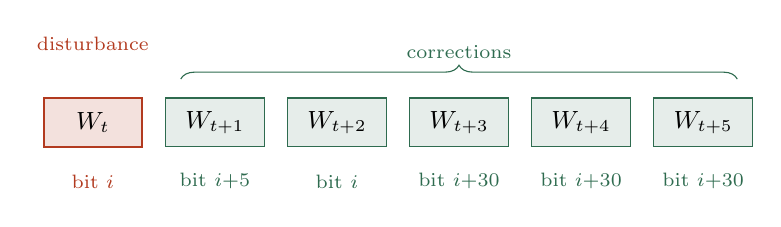
\begin{tikzpicture}[x=1.55cm,y=1cm,>=Stealth,
  w/.style={draw,minimum width=1.25cm,minimum height=0.62cm,font=\small}]
  \node[w,fill=disturb!15,draw=disturb,thick] (w0) at (0,0) {$W_t$};
  \foreach \i/\lbl in {1/{W_{t+1}}, 2/{W_{t+2}}, 3/{W_{t+3}}, 4/{W_{t+4}}, 5/{W_{t+5}}}
    \node[w,fill=correct!12,draw=correct] (w\i) at (\i,0) {$\lbl$};

  \node[font=\scriptsize,disturb] at (0,-0.75) {bit $i$};
  \node[font=\scriptsize,correct] at (1,-0.75) {bit $i{+}5$};
  \node[font=\scriptsize,correct] at (2,-0.75) {bit $i$};
  \node[font=\scriptsize,correct] at (3,-0.75) {bit $i{+}30$};
  \node[font=\scriptsize,correct] at (4,-0.75) {bit $i{+}30$};
  \node[font=\scriptsize,correct] at (5,-0.75) {bit $i{+}30$};

  \node[font=\scriptsize,disturb,align=center] at (0,1.0) {disturbance};
  \draw[decorate,decoration={brace,amplitude=5pt},correct]
    (0.72,0.55) -- (5.28,0.55)
    node[midway,above=4pt,font=\scriptsize,correct] {corrections};
\end{tikzpicture}
\caption{One local collision. The offsets are not arbitrary: $+5$ undoes the
$\rotl^{5}(a)$ of the following round, and the three $+30$s track the bit as
$\rotl^{30}$ carries it through register $c$ (Figure~\ref{fig:round}). The
same six-word pattern is what \texttt{add\_local\_collision} in
\texttt{broken/attack/collide.c} writes.}
\label{fig:local}
\end{figure}

The cancellation is not free. The round adds modulo $2^{32}$ while the
differential is stated in XOR, and $f_t$ may or may not pass the difference
through. \texttt{collide verify} measures how often it works, over 200\,000
random states per row:

\begin{center}
\begin{tabular}{llrr}
\toprule
rounds & $f_t$ & $i=1$ & $i=2$ \\
\midrule
0--19  & Ch     & 0.0157 & 0.0027 \\
20--39 & Parity & \textbf{0.1242} & 0.0167 \\
40--59 & Maj    & 0.0152 & 0.0029 \\
60--79 & Parity & \textbf{0.1247} & 0.0169 \\
\bottomrule
\end{tabular}
\end{center}

Two things follow, and both were corrected \emph{by} the measurement rather
than confirmed by it.

\paragraph{The Parity rounds are cheaper but not free.} It is often said that
a linear $f$ makes a local collision cost nothing. The measurement says
$\approx 2^{-3}$, about eight times cheaper than the nonlinear rounds and not
free at all. The reason is worth stating precisely: making $f$ linear removes
the conditions \emph{on $f$}, and what is left is the additions. Equation
\eqref{eq:round} adds modulo $2^{32}$, so an XOR correction is exact only when
no carry crosses the corrected bit. That residual is the $2^{-3}$.

\paragraph{Bit 1 is the right place to work.} Bit 1 beats bit 2 by the same
factor of eight, for the same reason: the corrections sit at $i+5$ and $i+30$,
and at $i=1$ the $i+30$ corrections land at bit 31, where a carry out of the
top is discarded instead of propagating. Every disturbance vector in the
literature uses bit 1, and this is why.

% ===========================================================================
\section{Disturbance vectors, and a condition that is easy to miss}
\label{sec:dv}

A single local collision is not a collision of the hash: the message
difference it needs must itself be producible by the expansion. So the
attacker picks a codeword of the code in \S\ref{sec:buys} --- the
\emph{disturbance vector} --- and places one local collision at every round
where it is set. Its weight is the number of local collisions to be paid for,
so low weight is the whole game, and the last five rounds must be quiet
because a disturbance at round $R-1$ cannot be corrected before the block
ends.

There is a further condition, and omitting it is not a small mistake. The
message difference in a given bit column is a sum of \emph{time-shifted}
copies of the disturbance vector, one per correction offset. Every one of
those shifts has to be a codeword in its own right. A shift by $k$ satisfies
\eqref{eq:scalar} only from round $16+k$ onwards, so requiring shifts $1$
through $5$ to be codewords imposes $1+2+3+4+5 = 15$ extra linear conditions.

That is not vacuous: it cuts the $65\,535$ nonzero codewords down to
$\mathbf{2047}$, a subspace of dimension 11. The first version of
\texttt{broken/attack/collide.c} left the condition out and reported
\texttt{difference is a valid expansion: NO} for every round count --- the
differential was not merely unlikely, it was unmountable. With the condition
imposed the same program finds collisions immediately.

% ===========================================================================
\section{What actually runs here}\label{sec:runs}

\texttt{collide search} builds the message difference from a disturbance
vector and searches for a message pair on which every local collision happens
to cancel. Both messages are exactly one 64-byte block, so they pad
identically and a collision in the first compression is a collision of the
whole hash --- not merely of the compression function.

\begin{center}
\begin{tabular}{rrrr}
\toprule
rounds & DV weight & result & time \\
\midrule
20 & 3 & collision & $<0.1$\,s \\
25 & 3 & collision & $<0.1$\,s \\
30 & 7 & not found in 25\,s & --- \\
40 & 12 & not found in 25\,s & --- \\
\bottomrule
\end{tabular}
\end{center}

A collision found on the machine this was written on, and re-verified through
the command-line tool rather than trusted from the search:

\begin{lstlisting}
m1 = a0ff9c057ffb967705882f6996497503caa75b02710d381205465e6257897d37
     d8e7937059d6088b323f31b7986989ed0ba3ef5dc0d1bf15bb2ffd82420a7f32
m2 = a0ff9c057ffb967705882f6996497503caa75b02710d381205465e6057897d77
     d8e79372d9d6088bb23f31b7186989ed0ba3ef5dc0d1bf15bb2ffd80420a7f72

SHA0-25(m1) = 6b967bd82efc21d8011755a15a10a2e7200a9094
SHA0-25(m2) = 6b967bd82efc21d8011755a15a10a2e7200a9094
\end{lstlisting}

\noindent
At full 80 rounds the same two messages hash to
\texttt{9a276e8d...} and \texttt{ccbaa7e1...}: different, as they must be.

Beyond about 25 rounds the search needs \emph{message modification} --- fixing
up the early rounds deterministically instead of waiting for random messages
to satisfy them --- which is what Wang's work supplied and what this
implementation does not have. That is the honest boundary of what is here.

% ===========================================================================
\section{The history}\label{sec:history}

\begin{figure}[h]
\centering
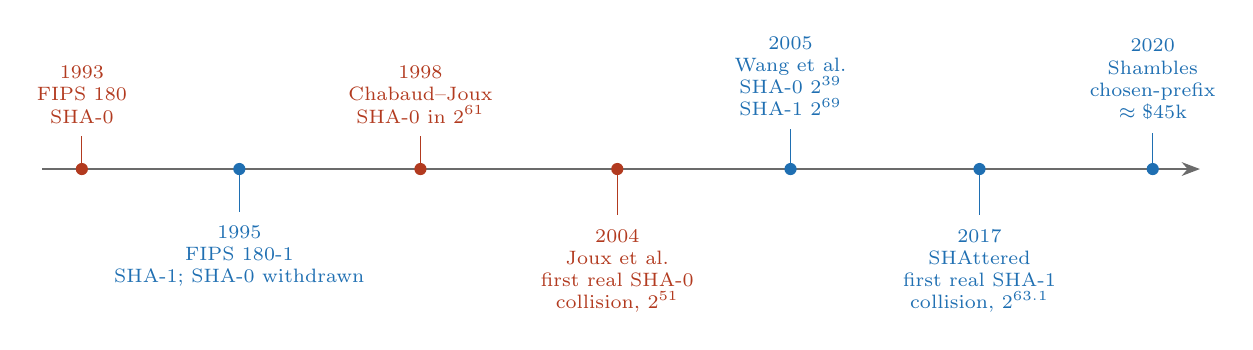
\begin{tikzpicture}[x=1cm,y=1cm,>=Stealth]
  \draw[->,softgrey,thick] (-0.5,0) -- (14.2,0);
  \foreach \x/\y/\lbl/\col in {
      0/1.0/{1993\\FIPS 180\\SHA-0}/sha0col,
      2/-1.3/{1995\\FIPS 180-1\\SHA-1; SHA-0 withdrawn}/sha1col,
      4.3/1.0/{1998\\Chabaud--Joux\\SHA-0 in $2^{61}$}/sha0col,
      6.8/-1.4/{2004\\Joux et al.\\first real SHA-0\\collision, $2^{51}$}/sha0col,
      9/1.2/{2005\\Wang et al.\\SHA-0 $2^{39}$\\SHA-1 $2^{69}$}/sha1col,
      11.4/-1.4/{2017\\SHAttered\\first real SHA-1\\collision, $2^{63.1}$}/sha1col,
      13.6/1.1/{2020\\Shambles\\chosen-prefix\\$\approx\$45$k}/sha1col} {
    \fill[\col] (\x,0) circle (2.2pt);
    \draw[\col] (\x,0) -- (\x,\y*0.42);
    \node[\col,font=\scriptsize,align=center,anchor=\ifdim\y pt>0pt south\else north\fi]
      at (\x,\y*0.46) {\lbl};
  }
\end{tikzpicture}
\caption{Twenty-seven years. The gap between the two red clusters and the two
blue ones is what the rotation of \eqref{eq:exp1} bought.}
\label{fig:timeline}
\end{figure}

\textbf{1993--1995.} NIST published SHA-0, then withdrew it two years later
and replaced it with SHA-1, saying only that a design flaw had been found. No
technical justification was published at the time.

\textbf{1998.} Chabaud and Joux introduced local collisions and disturbance
vectors and gave a $2^{61}$ attack on the SHA-0 compression
function~\cite{chabaud1998}. Their abstract already records the punchline of
this document: the same method ``is unable to find collisions faster than the
birthday paradox'' for SHA-1, which they call strong evidence that the
rotation was added for exactly this reason.

\textbf{2004.} Joux, with Carribault, Lemuet and Jalby, found the first actual
SHA-0 collision on a 256-CPU machine~\cite{joux2004}.

\textbf{2005.} Wang, Yu and Yin reduced SHA-0 to about
$2^{39}$~\cite{wang2005sha0} and, with the same machinery, gave the first
attack on full SHA-1 below the birthday bound at about
$2^{69}$~\cite{wang2005sha1}. SHA-1 was theoretically broken from that moment
and remained in wide deployment for another twelve years.

\textbf{2017.} SHAttered produced two PDF files with the same SHA-1, at a cost
of roughly $2^{63.1}$ compressions~\cite{stevens2017}.

\textbf{2020.} Leurent and Peyrin gave the first \emph{chosen-prefix}
collision for around \$45{,}000 of rented GPU time~\cite{leurent2020}. A
chosen-prefix collision is the one that matters operationally: it lets an
attacker collide two documents each of which begins however they like.

% ===========================================================================
\section{What is not here}\label{sec:limits}

\begin{itemize}[leftmargin=1.4em]
\item \textbf{No full SHA-0 or SHA-1 collision.} Those cost about $2^{39}$ and
      $2^{63}$ and are not reachable on one machine in one session. Nothing in
      \texttt{broken/} claims otherwise.
\item \textbf{No message modification.} \S\ref{sec:runs} stops around 25
      rounds for want of it.
\item \textbf{No historic collision data.} The SHAttered blocks are not
      embedded; the paper is cited and mirrored instead.
\item \textbf{No SHA-0 oracle exists.} SHA-1 is checked here against three
      independent implementations. SHA-0 is implemented by nothing current, so
      it rests on published known-answer vectors plus the structural check
      that switching the rotation on turns every SHA-0 answer into the
      oracle-verified SHA-1 one.
\item \textbf{Neither function is safe to use.} That is the point of the
      document.
\end{itemize}

\printbibliography[heading=bibintoc]

\end{document}
